% This must be in the first 5 lines to tell arXiv to use pdfLaTeX, which is strongly recommended.
\pdfoutput=1
% In particular, the hyperref package requires pdfLaTeX in order to break URLs across lines.

\documentclass[11pt]{article}

% Remove the "review" option to generate the final version.
\usepackage[]{ACL2023}

% Standard package includes
\usepackage{times}
\usepackage{latexsym}
\usepackage{graphicx} 

% CUSTOM PACKAGES
\usepackage{pgfplots}
\pgfplotsset{width=10cm,compat=1.9}
\usepackage{tikz}
\usepackage{subcaption}
\usepackage{fontawesome5}
\usepackage{tikz-cd}
%\usepackage[dvipsnames]{xcolor}


\usepackage{soul}
% For proper rendering and hyphenation of words containing Latin characters (including in bib files)
\usepackage[T1]{fontenc}
% For Vietnamese characters
% \usepackage[T5]{fontenc}
% See https://www.latex-project.org/help/documentation/encguide.pdf for other character sets

% This assumes your files are encoded as UTF8
\usepackage[utf8]{inputenc}

% This is not strictly necessary, and may be commented out.
% However, it will improve the layout of the manuscript,
% and will typically save some space.
\usepackage{microtype}

% This is also not strictly necessary, and may be commented out.
% However, it will improve the aesthetics of text in
% the typewriter font.
\usepackage{inconsolata}


\tikzset{
    lm-bg halfcircle/.style={%
        mark=halfcircle*,
        mark color=teal!75!white,
        every mark/.append style={rotate=#1}
    }
}
\tikzset{
    mt-bg halfcircle/.style={%
        mark=halfcircle*,
        mark color=Salmon!75!white,
        every mark/.append style={rotate=#1}
    }
}


\newcommand{\bs}[1]{\textcolor{black}{#1}}
\newcommand{\mn}[1]{\textcolor{black}{#1}}
\newcommand{\ar}[1]{\textcolor{black}{#1}}
\newcommand{\lb}[1]{\textcolor{black}{#1}}
%\newcommand{\todo}[1]{\textcolor{pink}{#1}}

\usepackage{todonotes}
\usepackage{soul} % for \ul and \TODOMARK
\usepackage{marginnote}
\usepackage{url}
\let\marginpar\marginnote

\usepackage[capitalize]{cleveref}

\usepackage{listings}
\lstset{breaklines=true, % Enable automatic line breaking
        basicstyle=\ttfamily, % Use typewriter font
        xleftmargin=0pt, % Remove left indentation
        frame=none, % No frame around the code
        numbers=none} % No line numbers


\definecolor{TodoColor}{rgb}{1,0.7,0.6}
\definecolor{TodoColor2}{rgb}{0.7,0.7,0.9}
\definecolor{TodoColor3}{rgb}{0.5,0.8,0.5}
\newcommand{\todonote}[3][]{\todo[color=#2,size=\scriptsize,fancyline,caption={},#1]{#3}}
\newcommand{\todox}[2][]{\todonote[#1]{TodoColor}{\textbf{TODO:} #2}}

% add here your initials for colorful comments
\newcommand{\bes}[2][]{\todonote[#1]{cyan!30}{\textbf{\textit{Todo}:} #2}}
\newcommand{\BS}[2][]{\bs[inline,#1]{#2}}
\newcommand{\mnc}[2][]{\todonote[#1]{red!30}{\textbf{\textit{Todo}:} #2}}
\newcommand{\lbc}[2][]{\todonote[#1]{blue!30}{\textbf{\textit{Todo}:} #2}}

% \newcommand{\TODO}[2][]{\todox[inline,#1]{#2}}
% \newcommand{\TODOMARK}{\textcolor{black}{\sethlcolor{TodoColor} \small \hl{\textbf{TODO}}}\xspace}

% If the title and author information does not fit in the area allocated, uncomment the following
%
%\setlength\titlebox{<dim>}
%
% and set <dim> to something 5cm or larger.


\title{Translation in the Hands of Many: \\
Machine Translation as a (Lay) User-Facing Technology}


\title{Translation in the Hands of Many: \\
Centering Lay Users in Machine Translation Interactions}

% Author information can be set in various styles:
% For several authors from the same institution:

% author{Beatrice Savoldi\textsuperscript{\textcolor{fem}{$\blacksquare$}}, Sara Papi\textsuperscript{\textcolor{fem}{$\blacksquare$}}, Matteo Negri\textsuperscript{\textcolor{fem}{$\blacksquare$}},\\ \textbf{Ana Guerberof Arenas\textsuperscript{\textcolor{masc}{$\bigstar$}}, Luisa Bentivogli\textsuperscript{\textcolor{fem}{$\blacksquare$}}} \\
%   \textsuperscript{\textcolor{fem}{$\blacksquare$}}Fondazione Bruno Kessler, Italy \\
%   \textsuperscript{\textcolor{masc}{$\bigstar$}}University of Groningen, Netherlands \\
%   \texttt{\{bsavoldi,spapi,negri,bentivo\}@fbk.eu} \\
%   \texttt{a.guerberof.arenas@rug.nl}}

  
\author{Beatrice Savoldi, Alan Ramponi, Matteo Negri, Luisa Bentivogli
         \\ Fondazione Bruno Kessler, Italy \\
         \texttt{\{bsavoldi,alramponi,negri,bentivo\}@fbk.eu}}
% if the names do not fit well on one line use
%         Author 1 \\ {\bf Author 2} \\ ... \\ {\bf Author n} \\
% For authors from different institutions:
% \author{Author 1 \\ Address line \\  ... \\ Address line
%         \And  ... \And
%         Author n \\ Address line \\ ... \\ Address line}
% To start a seperate ``row'' of authors use \AND, as in
% \author{Author 1 \\ Address line \\  ... \\ Address line
%         \AND
%         Author 2 \\ Address line \\ ... \\ Address line \And
%         Author 3 \\ Address line \\ ... \\ Address line}

% \author{First Author \\
%   Affiliation / Address line 1 \\
%   Affiliation / Address line 2 \\
%   Affiliation / Address line 3 \\
%   \texttt{email@domain} \\\And
%   Second Author \\
%   Affiliation / Address line 1 \\
%   Affiliation / Address line 2 \\
%   Affiliation / Address line 3 \\
%   \texttt{email@domain} \\}

\begin{document}
\maketitle
\begin{abstract}
Converging societal and technical factors
%--such as global interconnectedness, the explosion of digital content, and advances in core technology---
have transformed language technologies into user-facing applications employed 
%by millions 
across 
%numerous 
languages. 
%As a cornerstone task in NLP, 
Machine Translation (MT) has become a global tool,
%---virtually accessible to anyone with an internet connection--
%and 
with cross-lingual services now also supported by dialogue systems powered by multilingual 
Large Language Models (LLMs).    
This accessibility has expanded MT’s reach to a vast base of \textit{lay~users}, often with little to no expertise in the languages or the technology itself. Despite this,
%this ubiquity
the understanding of MT consumed by this diverse group of users%
%lay users%
% MT for the general public, and how it serves lay users
% the understanding of MT end users---particularly lay users
---their needs, experiences, and interactions with these systems---remains limited. 
%Questions persist regarding how effectively MT addresses real-world challenges and incorporates human factors into its design. 
%This paper examines the evolution of MT usage and user profiles, 
%
This paper traces the shift in MT user profiles, focusing on non-expert users and how their engagement with these systems may change with LLMs. We identify three key factors---usability, trust, and literacy---that shape these interactions and must be addressed to align MT with user needs. By exploring these dimensions, we offer 
insights 
%and 
%recommendations 
to guide future MT 
%solutions 
with a user-centered approach.


% In this paper, we first trace the evolution of MT usage and user profiles by examining the shift to non-expert users, and how their interactions with these systems might further change with the advent of LLMs. 
% We identify three key factors---usability, trust, and literacy---that 
% shape these interactions and 
% must be addressed to better align MT with the needs of lay end-users. By exploring these dimensions, we provide insights and recommendations to incorporate them in future MT solutions 
% paired with user-centered considerations. 

%%%%%%%%%SHORTER ABSTRACT%%%%%%%%%%%
% Converging societal and technical factors have transformed language technologies into widely used, user-facing applications. Machine Translation (MT), now globally accessible, has expanded its reach to a diverse base of lay users with little to no expertise in translation. With the rise of multilingual Large Language Models (LLMs) integrated into dialogue systems, MT usage is evolving, yet our understanding of lay users’ needs, experiences, and interactions remains limited.





\end{abstract}

\section{Introduction}

% \bs{The success of technology hinges on its ability to serve users, and Natural Language Processing (NLP) faces this challenge as it moves from an academic pursuit to a set of impactful tools. Among them, MT stands out as a cornerstone application, with wide adoption fostered by its quality, the availability of online user-facing systems, and the growing need for multilingual communication \citep{WANG2022143, green2015natural}. Once confined to professional translation settings, MT is now used by millions worldwide \citep{pitman2021translate}, bringing into its fold a diverse array of lay users in contexts ranging from casual interactions \citep{robertson2022understanding} to critical domains such as healthcare and employment \citep{patil2014use, dew2018development, liebling-etal-2022-opportunities, valdez2023migrant}. 
% }

The success of technology hinges on its ability to serve users, and Natural Language Processing (NLP) confronts this challenge as it transitions from an  
academic pursuit to a set of 
%widely deployed, 
impactful tools. Among them, MT stands out as a cornerstone %NLP 
application,
%\footnote{We use ``MT’’ to refer to the task of automatically rendering content across languages, regardless of the core technology used to perform the task.} 
%whose breadth and quality fostered wider adoption
with current breadth and quality that  
fostered wider adoption \citep{WANG2022143}. 
%The need for multilingual communication 
Multilingual demands \citep{moorkens2024artificial},
% \footnote{The global translation service market was valued USD 41.78 billion in 2024 and is expected to grow: \url{https://straitsresearch.com/report/translation-service-market}.\bes{Questo punto suona piu' market oriented che user-oriented. Abbiamo altri dati migliori available?}} 
paired with the accessibility of online systems, has put MT at the forefront of user-facing language technologies.
%\citep{green2015natural}.
%, being used by millions worldwide  \citep{pitman2021translate}.
%
% MT, available beyond professional translation settings, MT has brought an increasingly diverse array of \textit{lay users} into its fold \todo{cit}, who rely on it or tasks ranging from casual interactions to critical scenarios like healthcare and employment \todo{cit}. 
%
% Its availability has extended beyond professional translation settings, bringing an increasingly diverse array of \textit{lay users} into its fold,  who rely on raw MT outputs for several activities ranging from casual interactions \citep{robertson2022understanding}, gisting content \citep{nurminen-papula-2018-gist}, to critical scenarios like healthcare and employment  \citep{patil2014use, dew2018development, liebling-etal-2022-opportunities, valdez2023migrant}.
%
Once confined to professional 
%translation 
settings, MT is now used by millions 
%worldwide
\citep{pitman2021translate}, bringing into its fold an 
%diverse 
array of \textit{lay users} in contexts ranging from casual interactions 
\citep{gao}
%\citep{robertson2022understanding} 
to critical domains such as healthcare and employment \citep{patil2014use, dew2018development, liebling-etal-2022-opportunities, valdez2023migrant}. 


\begin{figure}[!t]
%%%
\begin{subfigure}{.24\textwidth}
%%%
    \resizebox{\linewidth}{!}{%

    \begin{minipage}[t]{.99\linewidth}
    \centering
    \strut\vspace*{-9mm}\newline
    
        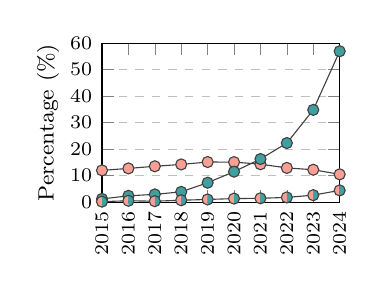
\begin{tikzpicture}
            \begin{axis}[
                /pgf/number format/1000 sep={},
                %xlabel={Publishing year},
                ylabel={Percentage (\%)},
                ylabel style={yshift=-1mm},
                %xmin=2000, xmax=2024,
                xmin=2015, xmax=2024,
                ymin=0, ymax=60,
                %xtick={2000,2005,2010,2015,2020,2025},
                xtick={2015,2016,2017,2018,2019,2020,2021,2022,2023,2024,2025},
                ytick={60,50,40,30,20,10,0},
                height=3.6cm,
                width=4.6cm,
                legend pos=north west,
                ymajorgrids=true,
                grid style=dashed,
                title style={yshift=-3mm},
                xlabel style = {font=\footnotesize},
                ylabel style = {font=\footnotesize},
                xticklabel style = {font=\scriptsize, rotate=90},
                yticklabel style = {font=\scriptsize},
                legend style={font=\scriptsize},
                % line width=0.2mm,
                % title={x}
            ]

            \addplot[
                color=Salmon!75!white,
                mark=*,
                draw=black!75!white,
                ]
                coordinates {
                %(2000,10.18)(2001,19.55)(2002,13.43)(2003,14.99)(2004,9.59)(2005,18.76)(2006,12.87)(2007,16.80)(2008,15.71)(2009,14.49)(2010,15.21)(2011,15.27)(2012,15.37)(2013,13.57)(2014,14.69)
                (2015,11.96)(2016,12.71)(2017,13.51)(2018,14.21)(2019,15.12)(2020,15.09)(2021,14.29)(2022,12.90)(2023,12.20)(2024,10.48)
                };
            %\addlegendentry{MT}

            \addplot[
                color=teal!75!white,
                mark=*,
                draw=black!75!white,
                ]
                coordinates {
                %(2000,0.92)(2001,1.71)(2002,0.86)(2003,1.53)(2004,1.02)(2005,2.16)(2006,1.91)(2007,1.62)(2008,2.23)(2009,1.58)(2010,1.34)(2011,2.01)(2012,1.93)(2013,2.09)(2014,2.10)
                (2015,1.19)(2016,2.36)(2017,2.91)(2018,3.86)(2019,7.31)(2020,11.48)(2021,16.25)(2022,22.28)(2023,34.81)(2024,56.94)
                };
            %\addlegendentry{LM}

            \addplot[
                color=Salmon!75!white,
                lm-bg halfcircle=90,
                draw=black!75!white,
                ]
                coordinates {
                %(2000,0.08)(2001,0.26)(2002,0.17)(2003,0.27)(2004,0.22)(2005,0.58)(2006,0.43)(2007,0.52)(2008,0.88)(2009,0.14)(2010,0.40)(2011,1.01)(2012,0.49)(2013,0.62)(2014,0.80)
                (2015,0.17)(2016,0.49)(2017,0.33)(2018,0.69)(2019,0.99)(2020,1.31)(2021,1.43)(2022,1.76)(2023,2.61)(2024,4.41)
                };
            %\addlegendentry{MT + LM}
            \end{axis}
        \end{tikzpicture}
        %\\

        \end{minipage}
}%
	%\caption{MT (red), LM (blue), MT+LM (green).}
	%\label{fig:trend}

%%%
\end{subfigure}%
\hfill
\begin{subfigure}{.24\textwidth}
%%%

    \resizebox{\linewidth}{!}{%

    \begin{minipage}[t]{.99\linewidth}
    \centering
    \strut\vspace*{-9mm}\newline
    
        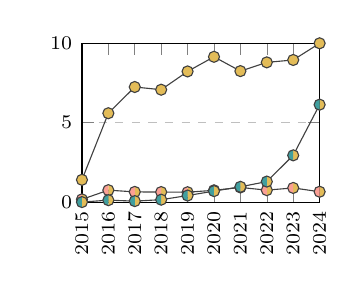
\begin{tikzpicture}
            \begin{axis}[
                /pgf/number format/1000 sep={},
                %xlabel={Publishing year},
                ylabel={\textcolor{white}{\%}},
                ylabel style={yshift=-3mm},
                %xmin=2000, xmax=2024,
                xmin=2015, xmax=2024,
                ymin=0, ymax=10,
                %xtick={2000,2005,2010,2015,2020,2025},
                xtick={2015,2016,2017,2018,2019,2020,2021,2022,2023,2024,2025},
                ytick={10,5,0},
                height=3.6cm,
                width=4.6cm,
                legend pos=north west,
                ymajorgrids=true,
                grid style=dashed,
                title style={yshift=-3mm},
                xlabel style = {font=\footnotesize},
                ylabel style = {font=\footnotesize},
                xticklabel style = {font=\scriptsize, rotate=90},
                yticklabel style = {font=\scriptsize},
                legend style={font=\scriptsize},
                % line width=0.2mm,
                % title={x}
            ]

            \addplot[
                color=Goldenrod!75!white,
                mark=*,
                draw=black!75!white,
                ]
                coordinates {
                %(2000,1.50)(2001,2.23)(2002,1.88)(2003,1.80)(2004,1.94)(2005,1.41)(2006,4.98)(2007,1.30)(2008,4.88)(2009,0.98)(2010,4.80)(2011,1.51)(2012,5.31)(2013,1.65)(2014,4.55)
                (2015,1.40)(2016,5.59)(2017,7.24)(2018,7.07)(2019,8.22)(2020,9.14)(2021,8.24)(2022,8.79)(2023,8.94)(2024,9.99)
                };
            %\addlegendentry{Users}

            \addplot[
                color=Goldenrod!75!white,
                mt-bg halfcircle=270,
                draw=black!75!white,
                ]
                coordinates {
                %(2000,1.00)(2001,1.71)(2002,0.77)(2003,0.81)(2004,0.75)(2005,0.75)(2006,0.72)(2007,0.26)(2008,0.74)(2009,0.14)(2010,0.57)(2011,0.59)(2012,1.20)(2013,0.15)(2014,0.91)
                (2015,0.17)(2016,0.75)(2017,0.64)(2018,0.63)(2019,0.62)(2020,0.74)(2021,0.92)(2022,0.75)(2023,0.89)(2024,0.65)
                };
            %\addlegendentry{MT + user}

            \addplot[
                color=Goldenrod!75!white,
                lm-bg halfcircle=270,
                draw=black!75!white,
                ]
                coordinates {
                %(2000,0)(2001,0)(2002,0)(2003,0)(2004,0)(2005,0)(2006,0.05)(2007,0)(2008,0)(2009,0)(2010,0)(2011,0)(2012,0)(2013,0)(2014,0.11)
                (2015,0)(2016,0.12)(2017,0.06)(2018,0.15)(2019,0.41)(2020,0.69)(2021,0.96)(2022,1.29)(2023,2.94)(2024,6.13)
                };
            %\addlegendentry{LM + user}
            \end{axis}
        \end{tikzpicture}
        %\\

        \end{minipage}
}%
	%\caption{Users (red), MT and users (blue), LM + users (green).}
	%\label{fig:trend2}
%%%
\end{subfigure}%
%%%

\caption{Trend of interest in \emph{machine translation} \colorbox{Salmon!75!white}{\textsc{\textbf{mt}}}, \emph{language models} \colorbox{teal!75!white}{\textsc{\textbf{\textcolor{white}{lm}}}}, \emph{users} \colorbox{Goldenrod!75!white}{\textsc{\textbf{u}}}, and combinations thereof in the ACL community over the last 10 years.\footnotemark}

\label{fig:trend-overview}

\end{figure}


Despite MT’s broad reach and potential for social impact in 
%increasingly 
sensitive scenarios \citep{vieira2021understanding}, still little is known about its evolving relationship with the general public, how non-expert %lay 
users interact with it, or how it caters to their needs. MT research has mainly focused on modeling advancements and%
% \footnote{With the goal of As \citet{Caselli} puts it, the generation of (human-like) text shall be regarded a mean to serve users, not as the end goal itself.}
---although translation studies have called for greater attention to end-user perspectives \citep{guerberof2023ethics}---MT works that actively involve lay people and 
%consider  
their experiences are 
still 
rare \citep{mehandru-etal-2023-physician, briakou-etal-2023-explaining, global-meeting}. 
%martindale2021machine, 
\footnotetext{Details on the ACL anthology queries are in Appendix~\ref{app:acl-query}.}

%In line with 
In the wake of broader calls to bridge MT \citep{liebling2021three} and language technologies with user-centered research \citep{heuer2021methods, kotnis2022human}, we posit that it is time to fill this gap and focus on how to support interactions between systems and lay people. 
% \emph{Why now?}\bes{If space allows, add other evidence of tracks/WS in the CL community to support argument (@Bea)} 
Arguably, the rise of powerful, instruction-following 
%prompt-based 
LLMs 
\citep[\textit{inter alia}]{touvron2023llama, achiam2023gpt, geminiteam2024geminifamilyhighlycapable, üstün2024ayamodelinstructionfinetuned}
engaging non-experts via chat interfaces has heightened user concerns (see Figure~\ref{fig:trend-overview}, 
%\textsc{lm+u}
%\textcolor{olive}{\textsc{\textbf{lm+u}}}
\colorbox{teal!75!white}{\textsc{\textbf{\textcolor{white}{lm}}}}+\colorbox{Goldenrod!75!white}{\textsc{\textbf{u}}}
on the \emph{right}) 
% \footnote{Trends based on publications in the ACL Anthology. For details on our queries see Appendix \ref{app:acl-query}.}
and underscores 
%and made more pressing 
the urgency to align with real-world interactions \citep{haque-etal-2022-pixie, liao2023aitransparencyagellms, szymanski2024comparingcriteriadevelopmentdomain}. 
As MT moves towards LLM-based solutions (see Figure \ref{fig:trend-overview}, 
%\textsc{mt+lm}
%\textcolor{olive}{\textsc{\textbf{mt+lm}}}
\colorbox{Salmon!75!white}{\textsc{\textbf{mt}}}+\colorbox{teal!75!white}{\textsc{\textbf{\textcolor{white}{lm}}}}
\emph{vs} 
%\textsc{mt} 
%\textcolor{magenta}{\textsc{\textbf{mt}}}
\colorbox{Salmon!75!white}{\textsc{\textbf{mt}}}
on the \emph{left}), these have the potential to redefine how people engage with multilingual systems, challenging traditional task divisions with new paradigms for cross-lingual communication \citep{ouyang2023shifted, lyu2024paradigm}. 

To set the stage for this shift towards lay users' perspective, we 
%first 
examine the evolution of MT from professional settings to its 
%growing 
wide general adoption (\S\ref{sec:mt-evolution}). We then identify three key factors---usability, trust, and literacy---to ground
%that are essential for 
%\bs{effective} \mnc{This is tricky: should we unroll the meaning of ``effective'' in a way that supports the three key factors chosen?}
user interactions with automatic translation tools (\S\ref{sec:factors}). Through this lens, we provide directions and recommendations to guide 
%future 
MT research in tandem with users (\S\ref{sec:recommendations}).



% =======================





%
% Investigations where MT is explicitly framed as a way to improve user lives are still scant, and although translation studies have called for greater attention to user perspectives \citep{guerberof2023ethics}, it rarely feeds back into the design of technology. Instead, MT research has largely focused on advancing model development to mimic language production rather than focusing on the evolving interaction between users and systems to make them meaningful and cater to user needs. 
%
%

% In light of the above, we align with broader calls to bridge MT \citep{liebling2021three, liebling-etal-2022-opportunities} and language technologies with user-centered research and HCI \citep{heuer2021methods, kotnis2022human}. By drawing on \bs{user research} \citep{schumacher2009handbook}, we examine the evolution of MT usage, with a focus on lay users, and identify three key factors—usability, trust, and literacy—that need to be considered for meaningful interactions with automatic translation tools.  Through this focus, we  provide insights and actionable recommendations for  future MT solutions in tandem with user research.





  



\section{MT Evolution: From Users to Uses} \label{sec:mt-evolution}
% MT for personal use emerged in the late 1990s with free online services,
% %like Babel Fish, 
% following the rise of personal computers and the Web \citep{yang1998systran, gaspari-hutchins-2007-online}. 
% Despite early reports of MT consumed by the public \citep{mccarthy2004does, somers2005round}, they represented secondary concerns. 
%
%\textbf{From professionals...} 
\textbf{Traditionally, real-world applications of MT have regarded so-called ``mixed MT'' workflows }\citep{wagner1983rapid}, where human intervention is required to revise---i.e. post-edit \citep{li2023post}---MT and ensure a reliable final translation.
% \bes{if space allows add that this use case was envisioned by Bar and clarify that this is still a realistic application (@bea)} 
With MT primarily consumed 
%and used
by \textit{professionals}, this context shaped its evolution \citep{church1993good}, influencing 
%system 
development \citep{green2014human, bentivogli2015evaluation, daems2019interactive}, %application 
interfaces~\citep{vieira2011review, vela2019improving}, and evaluation 
%criteria  
\citep{popovic2011towards, bentivogli2016neural}. 
Such a trajectory was also paired with 
%with 
empirical experiments on when MT could support \citep{koponen2016machine, moorkens2017assessing} or interfere \citep{federico2014assessing, daems2017identifying} with translators' activity.
%, to align and examine MT role for its intended audience and usage.
%
% \bes{If space allows, insert again=  Studies have examined how trust in MT affects adoption \citep{scansani2019translator}, which errors are most disruptive to translators (e.g., coherence issues being more problematic than local meaning shifts) \citep{federico2014assessing, daems2017identifying}, and the minimum quality threshold required for MT to actually support the translation workflow (). Similarly, \citet{turchi2015mt} explored whether quality estimation (QE) predictions of MT output quality could aid post-editors, as well as its potential and limitations in flagging word-level errors \citep{shenoy-etal-2021-investigating}. (@bea)}
Comparatively, despite early instances of MT for personal use \citep{mccarthy2004does, somers2005round}, 
%and online systems dating back to the 1990s \citep{yang1998systran, gaspari-hutchins-2007-online}, 
its availability to the general public remained limited and thus less of a concern. 

The advent of Transformer-based models with higher capabilities and expanded language coverage---along with the rise of the Web and 
%personal computers---altered
personal devices---altered 
this landscape.
\textbf{MT has now reached wider adoption by the general public, who directly accesses \textit{raw} MT output} in many diverse scenarios, e.g.
to gist content, for multilingual conversations \citep{conversation, pombal2024context}, in education \citep{yang2021measuring, yang2024understanding}, but also in high-stakes domains such as  healthcare \citep{khoong2019assessing}, migration 
%support 
\citep{liebling-etal-2022-opportunities}, and emergency services \citep{TURNER2015136}.\footnote{e.g. with COVID to compensate for interpreters shortages \citep{khoong2022research,anastasopoulos2020tico}.} 
%
\textbf{This shift} \textbf{to unmediated MT} 
%for the public 
\textbf{has led to a vast, heterogeneous base of \textit{lay users}}
% \footnote{\bs{Before considered end-users, or indirect stakeholders, which received post-edited text.}} 
\textbf{and, with it, novel desiderata and concerns}. For one, since lay users may have limited to no proficiency in at least one of the involved languages,\footnote{e.g. the \emph{source} language in gisting and the \emph{target} in communication contexts. See also \citet{nurminen-papula-2018-gist}.} they are more vulnerable to errors. 
%MT is not infallible: 
Mistranslations can lead to discomfort, misunderstandings, and even life-threatening errors \citep{taira2021pragmatic} and arrests \citep{guardian2017facebook}.
Besides, non-experts 
%usages and 
%users 
can have requirements and expectations of which little is known, and 
%in realistic settings 
that cannot be directly informed by existing research on professionals, as shown in the context of LLMs \citep{szymanski2024comparingcriteriadevelopmentdomain}. 

Indeed, 
%the rise of 
general-purpose LLMs are calling for more considerations of users and real-world contexts of use, as demonstrated by surveys to understand how people interact with technologies, for which purposes and needs~\citep[\textit{inter alia}]{tao-etal-2024-chatgpt, Skjuve_Brandtzaeg_Følstad_2024, Kim_2024, STOJANOV2024100243, bodonhelyi2024userintentrecognitionsatisfaction, wang2024user, HYUNBAEK2023102030}. \textbf{Chat-based LLMs} have drawn in millions of users,\footnote{According to \href{https://www.reuters.com/technology/artificial-intelligence/openai-says-chatgpts-weekly-users-have-grown-200-million-2024-08-29/}{OpenAI}, in the summer of 2024 ChatGPT reached 200 millions weekly active users.} with their impressive \textbf{versatility and engaging interfaces that allow verbalizing requests, also for automatic translation} \citep{ouyang2023shifted}. As the MT field explores
%is progressively exploring 
such  LLM-based solutions \citep[\textit{inter alia}]{zhu2023multilingual, lyu2024paradigm, alves2024toweropenmultilinguallarge} and integrates MT %tasks 
into more complex systems, these solutions have the potential to reshape cross-lingual services 
%besides traditional tasks,\footnote{e.g. providing a translation while summarizing the initial content and adjusting the style over one or multiple requests.} 
and user engagement. 
%

While this transition unfolds, overdue research on the experiences of lay users in cross-lingual and MT settings is gaining urgency. Ease of access does not ensure effective or reliable interactions. 
%
% \bs{We argue that the current shift is bringing to the fore and adding urgency to overdue research on the experiences of lay users in cross-lingual and MT settings.\bes{All this conclusive part and argument is weak, but after multiple attempts still here I am. Any feedback welcome} 
% Ease of access does not ensure effective or reliable interactions. 
%As lay people become actual users, they must navigate its limitations without adequate guidance. 
%
% Yet, research on user behaviors, support mechanisms, and strategies to help users assess translation reliability remains insufficient. 
%\faHandPointer), Trust (\faCheck), and Literacy (\faBookOpen)
As a first step to fill this gap,
%toward along this path, 
we examine three desirable factors that help us ground user-oriented MT for lay users:
%bridge MT to its lay users: 
\emph{i)} how to align technology to them (\textit{usability \faHandPointer}), \emph{ii)} how to calibrate user--MT interactions (\textit{trust \faCheck}), and \emph{iii)} how to empower users towards MT (\textit{literacy} \faBookOpen). Through this lens, we examine and take stock of the current landscape. 
%
% As we navigate this dynamic field, we must prioritize understanding end users and human factors in their interactions with these models. By centering our attention on user needs, we can ensure that these powerful technologies effectively facilitate meaningful communication across languages.





\section{Three Factors for MT Lay Users} \label{sec:factors}
% \bs{We review current research distributed across NLP, machine learning subfields, translation studies and HCI through of the lens of three factors that help us ground user-oriented MT for lay users: Usability (\faHandPointer), Trust (\faCheck), and Literacy (\faBookOpen)}\bes{weak:  to review based on prior paragraph}
% We examine three factors that should ground user-oriented MT for the general public. 
%
\paragraph{\faHandPointer \space Usability}
%To be informative for users, 
MT assessments should be meaningful---i.e.~reflecting values and criteria that are important and understandable for lay people---as well as reflective of how helpful or \textit{usable}\footnote{Usability regards how effectively, efficiently, and satisfactorily users achieve their goals in a given context \citet{ISO9241-11}.}
% \footnote{Usability, as defined by  \citet{ISO9241-11}, regards how effectively, efficiently, and satisfactorily users achieve their goals, taking account of the context of use.} 
technology is in meeting their goals. 
% Indeed, MT evaluation is a critical component, as it sets priorities that feedback into  
% design. 
The field, however, tends towards performance-driven %evaluations 
%and 
leaderboards 
\citep{rogers2019leaderboards}, which have been criticized for pursuing abstract notions of \emph{accuracy} and \emph{quality} above the practical \emph{utility} of a model or other relevant values \citep{ethayarajh-jurafsky-2020-utility}.
%, e.g. \emph{fairness}~\citep{birhane-2022}.
%
These values are often contextual:
%. For instance,
\citet{parthasarathi-etal-2021-sometimes-want} discuss how %values 
%\textit{robustness}  to errors and 
%\textit{robustness} misspellings
\textit{robustness} to misspellings might be detrimental if using MT for learning. 
%as a learning tool. 
Also, \textit{faithfulness} is normally %assumed to be 
key to ``MT quality'', but in creative contexts 
%such
like
subtitling, \textit{enjoyability} may take precedence over 
%strict 
fidelity 
%to the source 
\citep{guerberof2024or}. 
%

Standard MT metrics 
%\citep{papineni2002bleu, snover2006study, rei-etal-2020-comet}
% ---whether neural \citep{rei-etal-2020-comet} or based on string matching \citep{papineni2002bleu, snover2006study}---
offer coarse
%\bes{if space allows, bring into a footnote MQM} 
scores of generic performance
to rank and compare \textit{models}, but are opaque and only 
assume to inform how useful the model is when embedded within the system the user interacts with
%with which the user interacts\bes{add not on human-like performance} 
\citep{liebling-etal-2022-opportunities}. 
And yet,  
lay people are only involved as 
%manual 
evaluators to provide  
% are invol
% tend to be involved in MT assessments only as manual evaluators (e.g. crowd-workers) for 
model-centric insights, rather than to inform their experiences \citep{saldias-fuentes-etal-2022-toward, savoldi-etal-2024-harm}.\footnote{This might be further aggravated with LLM evaluators, which have been suggested as a surrogate for human participants \citep{wang2024large, agnew2024illusion}.} Furthermore, %\citet{liao2023rethinking} argues that 
general-purpose LLMs now confront us with an ``evaluation crisis'' \citep{liao2023rethinking}, where existing methods and predefined benchmarks for modular tasks may be obsolete, failing to capture real-world downstream contexts. This raises the risk of widening the socio-technical gap, where evaluation practices lack validity and might diverge from human requirements in realistic settings.  
%
% Critical challenges thus emerge in order to reconcile the benefits of standardized automatic measures, informed by ecologically valid studies that align with realistic lay users' needs and usability criteria. 







\paragraph{\faCheck \space Trust} %\bes{to shorten}
To prevent over-reliance on automatic translations, lay users must calibrate an appropriate level of (dis)\textit{trust}. 
%This is often in contrast with inflated expectations in the field about 
Indeed, they risk accepting potentially flawed translations at face value, and trust may be misplaced when an output appears believable but is inaccurate—an issue that is especially harmful in high-stakes contexts \citep{mehandru-etal-2023-physician}.
%
Prior research on MT has shown that \textit{fluency} and \textit{dialogue flow} can falsely signal reliability \citep{martindale-etal-2021-machine, robertson2022understanding}, and LLMs amplify this issue with their overly confident tone, even when incorrect \citep{xiong2024llmsexpressuncertaintyempirical, trust}. As general-purpose models increasingly replace domain-specific applications, providing mechanisms for trust calibration becomes even more urgent \citep{deng2022generalpurposemachinetranslation, litschko-etal-2023-establishing}.
%
To harness the benefits of MT systems while avoiding over-reliance on flawed translations, lay users often resort to back-translation\footnote{i.e., automatically translating a text to a target language and then back to the source language.} as a strategy to improve confidence~\citep{back-2007, zouhar-etal-2021-backtranslation, mehandru-etal-2023-physician}. However, back-translation is often performed manually due to the lack of dedicated functionalities, and its soundness
%effectiveness as a sound practice 
remains debated.
%
Another critical factor in fostering appropriate trust is \textit{transparency}---e.g. communicating uncertainty and providing explanations~\citep{liao2023aitransparencyagellms}. While explainability work is growing \citep{ferrando2024primer}, ensuring that explanations are informative and digestible to lay users rather than just developers is not trivial. Moreover, how to effectively integrate such uncertainty signals into the development of translation systems and their user interfaces is still an open question.


\paragraph{\faBookOpen \space Literacy}
% Even though MT has improved in quality, it remains imperfect, with issues varying by context, language pair, and domain\todo{cit}---and even by gender \citep{savoldi-etal-2021-gender}. To make the best use of MT, users must be aware of its limitations and where it might be flawed or risky, so they can also implement control measures. This is often in contrast to the inflated expectations in the field regarding the capabilities of these models, which can lead to negative perceptions, reduced acceptance, and compromised trust in MT systems \citep{kocielnik2019will}. \todo{cit NMT and human-like parity}
MT-mediation, as a form of human-machine interaction \citep{green2015natural,o2012translation}, should also regard how lay users themselves play a role in improving interactions and 
apply control strategies to overcome MT limitations.
%
% Although MT-mediated communication has been approached as a form of human-machine interaction for professionals \citep{green2015natural,o2012translation}, little consideration has been given to how lay users can enhance this interaction and apply control strategies to overcome MT limitations. 
This requires critical agency rather than passive consumption.
%
In this area, prior work \cite{myabe} has shown that
preventing the display of potentially flawed translations 
%disregards user judgment and 
causes discomfort to users, indicating that 
%users 
they
prefer warnings and guidance over outright blocks. But warnings serve as an initial signal; 
%\citep{zhao-etal-2024-successfully}; 
then users
% ---constrained by little proficiency of the source or target language---
should know how to proceed in recovering from MT errors \citep{shin2013enabling}.
%
To address this, \citet{bowker2019towards} introduce the concept of MT \textit{literacy}, a digital skill to equip users with the knowledge 
%and strategies 
to interact more effectively with MT.\footnote{For online materials, see \url{https://sites.google.com/view/machinetranslationliteracy/}.} This includes pre-editing input text to mitigate common failures (e.g. using short sentences). %or active voice). 
While literacy workshops proved beneficial to students
%this approach proves beneficial in academic contexts 
\citep{Bowker01092020}, 
%extending these strategies beyond students to 
reaching more vulnerable populations and underserved languages remains a challenge \citep{Liebling}.
%
Focusing on target 
%language 
comprehension, \citet{robertson2021three} explore interfaces with dictionary access and assistive bots.\footnote{See the Lara system, integrating the two-box interfaces with a bot: \url{https://laratranslate.com/translate}.} While LLMs encourage participation through chat and interactive queries \citep{qian2024enabling}, their reliability in this role remains uncertain, as LLM-powered systems may impact cognitive attention required for critical engagement  \citep{zhai2024effects, lee2025impact}. Also, MT literacy must evolve to address new types of opportunities and failures introduced by LLMs, such as 
%hallucinations \citep{rawte-etal-2023-troubling} and 
cascading errors across multiple requests.
% ===========================================================
% To make the best use of MT, users must be aware of its limitations and where it might be flawed or risky, so they can also implement control measures.

% A key factor in overcoming MT’s limitations, and more generally in having more fruitful interactions with MT, is \textit{literacy}. If we consider MT as a form of human-computer interaction, it works best when users have a degree of knowledge about the system and are empowered to exercise their agency. This means users should engage actively with the technology rather than rely on it passively.

% \citet{bowker2019towards} introduced the concept of MT literacy, initially defined as understanding how MT works, its implications, and strategies for improving translation quality. While it was initially aimed at the academic community, we advocate for a broader application to the general public. MT literacy involves being an informed and critical user—thinking about whether, when, why, and how to use MT rather than simply copying, pasting, and clicking.
% %
% Crucially, MT literacy is tied to \textit{agency}; involving lay users as active participants is essential because the mere accessibility of MT does not guarantee its effective use.

% \citet{Bowker01092020} reports on a workshop with Chinese speakers that increased awareness of different MT tools and strategies. Participants learned that various online MT systems can exhibit different behaviors and results, and they were taught how to improve input to enhance output (e.g., using short sentences, consistent terminology, and the active voice). Additionally, awareness of MT biases can improve user expectations and decision-making. The workshop yielded positive results, with participants reporting increased knowledge and confidence in using MT. While not everyone can attend formal courses, online resources are available to help develop MT literacy---although they are mostly targeting students right now.\footnote{See \url{https://sites.google.com/view/machinetranslationliteracy/}.}

% Agency can also be fostered during MT use by communicating uncertainties in a model, which has been shown to improve success rates in achieving goals \citep{zhao-etal-2024-successfully}. \todo{Robertson}'s work explores interfaces that provide access to dictionaries and assistive bots to help users create better inputs. Other research investigates MT warnings for potential cultural misunderstandings, indicating that alerts can improve awareness and reduce misinterpretations \todo{cit}. In a different study \todo{(Maybe et al., 2010)}, a system was tested that only allowed accurate messages to be exchanged. However, this approach disregarded user judgment and caused discomfort, suggesting that users prefer warnings and interactive guidance over outright message blocking.

% What does literacy and agency mean for large language models (LLMs)? To a certain extent, agency is more encouraged through chat. However, there is still much we do not know about literacy in the context of LLMs. MT literacy extends to understanding that LLMs learn and adapt based on past inputs and that they face specific challenges, such as hallucinations and cascading errors (for example, translating, then shortening, then refining the style).

\section{Future Directions and Conclusion} \label{sec:recommendations}
To conclude, we examine directions for future research in 
%cross-lingual technologies---
traditional or LLM-based MT
that integrates lay user perspectives. 
We map such directions and corresponding recommendations to the three factors outlined in section §\ref{sec:factors}. 
% In this work, we advocated for integrating user perspectives into cross-lingual technologies, whether traditional MT models or LLM-supported solutions. 
% To this end, we conclude by outlining a roadmap for a research agenda that integrates the user perspective and refocuses on user-centred MT research. We associate our recommendations and directions with the three factors outlined in the previous section (§\ref{sec:factors}). 

\paragraph{Consider Lay People As Users (\faHandPointer, \faCheck, \faBookOpen)} 
% To guadge of how and when users interact with MT, their attitudes toward the technology, and potential missed opportunities, we should consider their experiences as users rather than solely involve them as manual evaluators. 
% % Approaches that analyze user logs could be a first step to 
% observe real user engagement and preferences.
% Surveys and qualitative research can instead yield insights into their perceptions of MT and LLM-based cross-lingual services. Critically, research should be cautious to avoid two major pitfalls: \textit{i)} adopt an exploitative approach (\S\ref{sec:ethics}) or
% \textit{ii)} treat lay users as a homogeneous group. Critically, sociodemographics, education, background, and human factors such as the level of stress can influence user expectations, desires, and needs.  
%
To gauge how/when users interact with MT as well as current blindspots 
%\hl{missed opportunities,} 
%and their attitudes toward it, 
we should consider their experiences rather than just involve them as manual evaluators. Inspired by monolingual work \citep{handaeconomic},  analyzing user logs can help us observe real engagement and preferences. Surveys and \textit{in vivo} research offer qualitative insights into users' perceptions \citep{zheng, robertson2022understanding}. To this aim, it is essential to avoid two main pitfalls: \textit{i)} exploiting participants (see \S\ref{sec:ethics}) and \textit{ii)} treating them as a homogeneous group: 
%with the same goals: 
factors like sociodemographics, education, and stress levels can greatly influence their expectations and interactions \citep{rooein2023know, ai-culture}.


\paragraph{Design for Usability and Utility} (\faHandPointer)
Achieving human-like translations should not be blindly viewed as the ultimate goal---automated text is a means to serve a broader purpose, not an end in itself \citep{caselli-etal-2021-guiding}. 
%oward usability-based assesment for people, 
Prior work has evaluated systems based on their success in guiding human decision-making
%\footnote{i.e. instead of on the human-likeness of the automatic suggestions.}, 
%by measuring how successful they were at guiding humans in decision-making 
\citep{zhao-etal-2024-successfully} or by assessing gender bias in MT via user-relevant measures, like time, effort, or economic costs \citep{savoldi-etal-2024-harm}. Research could focus on making measurements more actionable \citep{delobelle-etal-2024-metrics}, e.g. to identify usability thresholds below which MT is no longer beneficial.
%\footnote{Similar efforts have been carried out for translators in MT \citep{turchi-etal-2013-coping}.}. 
Therefore, we should aim to correlate automated approaches with human-centered measurements to harness the benefits of both.\footnote{e.g. replicability and ecological validity, respectively.} 
 However, this is challenging due to the variability of utility values among users and usages. 
%this is challenging because utility values across users and uses can be diverse and thus hard to reconcile. 
Multi-metric and multifaceted approaches like HELM \citep{bommasani2023holistic}
show promise in this area, but future work could further align MT evaluation and design with socio-requirements and prototypical use cases \citep{liao2023rethinking}. 


% Future research should focus on making these measurements more actionable \citep{delobelle-etal-2024-metrics}, such as identifying usability thresholds below which MT becomes less effective\footnote{Similar efforts exist for translators in MT \citep{turchi-etal-2013-coping}.}. We should aim to correlate human-centered measurements with automated approaches to harness their combined benefits in realistic studies. However, this is challenging due to the variability of utility values among users. Multi-metric approaches like HELM \citep{bommasani2023holistic} show promise, but future work could better align evaluations and MT design with real user requirements and use cases \citep{liao2023rethinking}.


% further work could distill e.g., taxonomies of prototypical use cases and socio-requirements that can guide the evaluation methods to align them further to lay users. 

% Lay users are highly heterogeneous, making it difficult to reconcile their behaviors and needs within a single score. 

% It is essential to remember that human-like translations are not the ultimate goal—automated text is a tool to achieve a broader purpose. Instead of solely evaluating translation accuracy against professional standards, we should measure success based on real-world effectiveness.
% For instance: i) Daumé, in the context of visual grounding, assesses effectiveness by measuring whether users reach their intended destination rather than just the quality of the model’s directional suggestions. ii) Savoldi, in studying gender bias, emphasizes metrics that resonate with users, such as time, effort, or economic costs associated with biases. Also, Delobelle argues that metrics should be actionable—should they define a usability threshold beyond which a system should not be used? Konecke made an attempt, but their usability threshold was estimated rather than verified. Existing estimates in professional translation must also be adapted for lay users.
% Lay users are highly heterogeneous, making it difficult to reconcile their behaviors and needs within a single score. However, an essential first step is exploring key variables and correlating them with existing measurements.
% %
% Fro monolingual tasks, HELM represents an effort in this direction. It promotes multi-metric measurements, considering factors like robustness, efficiency, bias, and task-specific needs (e.g., factual consistency for summarization). Such multi-metric approaches cover more facets, but further work 
% distilling principles and representations (e.g., taxonomies of prototyp ical use cases and socio-requirements) that can guide the evaluation methods to align them further. 
% %It studies user needs, values, and downstream use cases to distill principles and taxonomies that guide ML evaluations.


\paragraph{Enrich MT Outputs} (\faCheck)
In user-facing systems, it is crucial to not only focus on generated translations but also to develop methods for \textit{estimating} and \textit{conveying} uncertainty, ambiguities, and errors to ensure reliable usage \citep{xu-etal-2023-understanding,zaranis-etal-2024-analyzing}.
%We advocate for ongoing efforts in explanability research to identify critical information on model rationale \citep{xu-etal-2023-understanding,zaranis-etal-2024-analyzing} and that could support users. 
For instance, \citet{briakou-etal-2023-explaining} use contrastive explanations to help users understand cross-linguistic differences, but it is unclear how to disentangle when their approach captures critical errors or simple meaning nuances in the wild. 
% For instance, \citet{briakou-etal-2023-explaining} explains cross-linguistic differences via contrastive explanations to align with human cognition, but in the wild it is hard to disentagle if their approach is sensitive to any meaning difference or actual errros. 
Quality estimation can also warn users in real time about flawed translations, though numeric indicators are hard to interpret to lay users \citep{inaccurate-message}. Indeed, a key area of future research is how to best communicate digestible information to lay users, e.g. via visualizations.\footnote{e.g. by highlighting errors or reliable keywords.} Textual explanations show promise in communicating uncertainty and avoiding over-reliance in LLMs, but the exact language used is relevant \citep{kim2024m}, and we thus advocate for MT work in this area. 

% Ultimately, a key area of research is finding how to convey this information clearly without overwhelming users, whether through visualizations or natural language explanations. The wording used in these communications is essential for effectiveness.

% Future research should shift from developer-focused information to user-friendly explanations that are clear and relatable. This remains a challenge in machine translation, with recent efforts using explainable AI (XAI) to identify hallucinations. For example, Briakou offers insights into cross-linguistic differences and detects errors through contrastive explanations, but its real-world application may not fully address all meaning differences.
% Quality estimation is another important research avenue. These models could warn users about low-quality outputs, but their effectiveness depends on the languages involved and the mode of communication. Studies indicate that numeric quality indicators often do not help users correct translation errors effectively.
% Ultimately, a key area of research is finding how to convey this information clearly without overwhelming users, whether through visualizations or natural language explanations. The wording used in these communications is essential for effectiveness.

%Future work in this area need to bridge from developer oriented information to something that is actually informative for users, e.g. and explanation that can be digestible, and pinpointed or relevant parts, align with human rationales, and can be useful in practice. This is an open challenge in MT, e.g. work in this area seek to use xai to identify hallucinations \citep{xu-etal-2023-understanding,zaranis-etal-2024-analyzing}. Briakou help user understand cross-lingual differences and detect errors via contrastive explanations, of phrses, that , once deleted, maximizes the model’s prediction. However, such an approach in the wild does not really disentagle e explanandum is sensitive to detecting any meaning differences and not only critical errors. 
%Quality estimation is also a direction
%To detect errors QE models  could warn users of low-quality outputs in real-time, though the quality of such models right now highly depend on the accounted languages, + how to communicate: Studies suggest that numeric quality indicators may not help users effectively correct translation errors,
%Indeed, a critical area of research also concerns how to best communicate this info ina digestible manner without overwhelming users, via visualization (e.g. highlt errros or keywords with high confidence?) or natural language explationas, %But how to communicate, with visualizations, scores or text is hard, as current studies shows that exact phrasing and language is very relevant \citep{kim2024m}

% Our findings suggest that using natural language expressions of uncertainty may be an effective approach  for reducing overreliance on LLMs, but that the precise language
%  used matters



%\bs{cit eamt} 
% and via interfaces. We advocate for increasing efforts in this direction to ensure reliable and trustworthy MT usage. 
% Still, caution is needed: explanation mechanisms in chat-based models may lead to over-reliance due to their overly persuasive nature and tone. 
% Concerning visualizations, it is debated whether it is more beneficial to lay users to highlight keywords with high chance of being correct, or rather error spans. Similarly, prior work has explored providing quality estimation scores to improve user trust, but numerical scores might be hard to interpret. 
% Ultimately, users should have realistic expectations of AI, avoiding claims of human-like parity and exaggerated capabilities.

% Translation is not an exact science, and MT is inherently imperfect. For sustainable and productive MT usage, users should be given more information—whether regarding interactions or two-box modes.
% This requires advancements in uncertainty and ambiguity detection, providing users with insights into system reliability. However, caution is needed: explanation mechanisms in chat-based models may lead to over-reliance due to their persuasive nature.
% Further exploration is needed on how to present quality estimation (QE) to users. Should it be in the form of scores? Are those scores intelligible? Would textual explanations be more effective? Research suggests that, while professional translators benefit from error highlighting, lay users may find it more helpful to visualize and emphasize reliable keywords instead (X).
% 

\paragraph{Foster Transparency (\faCheck \space \faBookOpen) and Agency (\faBookOpen)}
%
Effective interactions require users to be more than passive recipients of MT.
Besides real-time explanations, users should receive transparent information on the strenghts and limits of MT 
%in advance 
(e.g.~varying service across languages).
% and bias presence). 
%so as to contextualize general-purpose models. 
Thus, the field could adapt best practices for transparency 
%and accountability 
like  \textit{model cards} \citep{mitchell-2019} into simplified versions for the public, and contribute to literacy efforts on emergent technologies.% 
%and \textit{data statements} 
\footnote{e.g. see the ambitious Elements of AI program: \url{https://www.elementsofai.com/}.}
To foster agency, future work could explore how to address the found trade-off between the preference of some users
%\textit{\hl{some}} users' preference 
for riskier interactions versus more reliable ones, yet requiring their critical attention \citep{bucina}. 
Here, gamification \citep{Chen14122023} could be explored as a way to both enhance literacy and more enjoyable critical engagement.  
%While these efforts may seem distant, 
Experts in MT/NLP are best positioned to disseminate this knowledge by collaborating with other expertise. 
%They should collaborate with other communities to enhance transparency and foster informed usage.

% future work should explore how gamification

% Users are participants, not passive recipients. Effective interaction requires that they understand the minimal requirements and limitations of AI technology—across domains, languages, and contexts. Currently, evaluations rely on aggregate scores, making it difficult to pinpoint specific weaknesses on underserved domains, languages .
% In the field, initiatives like MT literacy and Finland’s AI literacy programs are emerging. Gamification has also been explored as a means to enhance cognitive capacity and user engagement in learning about AI systems. Research shows that increased exposure improves user understanding. However, there is a trade-off: some users prefer riskier interactions over cognitive forcing functions that push them to assess outputs critically.
% Future work should explore how gamification can aid engagement, such as using chatbots that prompt users for further input (e.g. Lara model). For experts, model cards exist—but what about simplified, digestible versions for lay users?
% While these efforts may seem distant, experts in MT/NLP are best positioned to disseminate this knowledge. They should collaborate with other communities to enhance transparency and foster informed usage.

\paragraph{Bridge Interdisciplinary Avenues (\faHandPointer, \faCheck, \faBookOpen})
Incorporating user needs, values, desiderata, and human factors is still in its early stages in NLP. However, disciplines like HCI, experimental psychology, and social sciences have established 
%human-centered  
practices to draw from \citep{liao2023rethinking}.
%that can be adapted. The same applies to gamification research.
These methodologies may take longer to implement, but they yield useful insights, e.g. on people cognition and trust, or to implement user studies.  
Besides, they offer methods that approximate real-world interactions cost-effectively, e.g. Wizard of Oz tests prior to developing a new method \citep{goyal-etal-2023-else}, or simulating user actions based on past user data \citep{zhang}. These approaches can be highly useful, but---circling back this section---the fundamental first step remains engaging with end users to understand their needs and behaviors first. 

% Circling back this section, such approaches require as a first step to have acquired knowledge and be informed by the behaviours and needs of actual users. 


% Also, HCI research has long developed cognitive models (Pirolli, 2007; Olson \& Olson, 1995; Card et al., 1983) to simulate user interactions, aiming to approximate real-world interactions cost-effectively. Circling back to the first avenue of future research, however, \lb{the first key step is grounding these simulations and inform them against real users, users' data, and usages.} 



% ===============================================================

% \paragraph{eval}
% \begin{itemize}
%     \item Improve lay user agency: foreground them and involve them as users and consumers of the technology, not just as crowdworkers and manual evaluators. 
%     \item Usability: Considering a shift from "quality" to "usability" is essential. Usability, as defined by ISO 9241-11 (ISO, 1998), measures how effectively, efficiently, and satisfactorily users achieve their goals. Bridging the gap between metrics and usability is crucial to align assessments and MT design to users. A potential direction is that of exploring how different usability criteria correlate with current automatic assessments and context and work on measurements that report them instead of one aggregated score.
%     \item Consider evaluations not only on the model, but on the entire system. This an impact as a variable and it is necessary to evaluate MT as a human-machine interaction and better understand how and why users need it. A viable approach that might be interesting, and which is gaining traction in the study of LLMs is that of collecting and exploring user logs---e.g. see \citet{}
%    % making MT reliable and accessible for end-users.
%     \item Rely on methods from HCI, User Research, Participatory to understand desiderata and limitations. People are not just data workers. Assess potential utilities and features with Wizard of OZ experiments, ethnographic and qualitative investigation, too. This is the starting point that could feed back into automatic evaluation modeling and system design. Understand that there are also limitations with involving people, and we should avoid exploitative approach---e.g. migrant women would not engage with survey on MT usage among migrant workers \citep{liebling-etal-2022-opportunities}. 
    
% \end{itemize}



% \section{Conclusion}

\section{Limitations}
\label{sec:limitations}


\paragraph{Slower science.} Our proposed future directions advocate for user-centered analyses and studies that require more time and resources compared to automated evaluations and \textit{in vitro} experiments, potentially slowing down the research cycle. However, we argue that user-driven insights are crucial and can only yield benefits to align MT with real-world needs and users. 

\paragraph{Factors.} Our analysis centers on three key criteria: \textit{usability, trust, and literacy}. These are not exhaustive of all user-centered concerns, but they serve as a starting point for a research agenda that encompasses user-machine interaction from distinct perspectives: \textit{usability} (model/system adaptation to users), \textit{trust} (the real-time interaction between users and technology), and \textit{literacy} (how users can play a role in engaging with and learning about MT). 

\paragraph{Text-to-Text MT.} We do not unpack the differences between text-to-text MT and other modalities, such as speech translation. While we acknowledge the relevance of these distinctions, we chose to focus on the broadest and most established MT technology. Expanding to other modalities is an important avenue for future work, but our scope was limited by space and focus.


\paragraph{ACL Anthology query} Our trends assessment of prior work on MT, LLMs, and Users---reported in Figure \ref{fig:trend-overview}---is based on papers published in the ACL Anthology (see Appendix~\ref{app:acl-query}). While including other sources could have further enriched our trend overview, the Anthology remains the main historical reference point in NLP. Hence, it represents an optimal litmus test for assessing trajectories in the field. Still, throughout the paper, we engage with literature from diverse communities, primarily from \textit{translation studies} and \textit{human factors in computing}, to provide a broader interdisciplinary perspective.


\section{Ethics Statement}
\label{sec:ethics}


In this work, we advocate for user-centered MT research by focusing on lay users. First, unlike human-in-the-loop methods \citep{wang-etal-2021-putting}---which rely on human contributions to enhance model functionality---we prioritize approaches and directions that are intended to serve and benefit users. 

Second, we do not conduct experiments with participants in this paper. Hence, we do not discuss ethical best practices for research in this area, though we deem them as indispensable e.g. obtaining proper ethical approval, securing informed consent, and ensuring non-intrusive engagement when working with human participants.

Finally, while we broadly discuss lay users, we do recognize that they actually encompass diverse groups and communities.  Many remain underserved by language technologies, particularly speakers of ``low-resource'' languages, and might face well-known biases in NLP tools related to gender \citep{savoldi-etal-2021-gender}, dialect \citep{blodgett-etal-2020-language}, or social class \citep{curry-etal-2024-classist}. Especially when engaging with more vulnerable communities and user groups, it is important to respect their lived experiences, avoid exploitative research practices, and ensure they are not treated as mere data sources but as valued participants and users---see e.g. \citet{bird-yibarbuk-2024-centering, ramponi-2024-language} and \citet{birhane2022power}.



\bibliography{anthology,custom}
\bibliographystyle{acl_natbib}

\newpage

\appendix

\section*{Appendix}

\section{ACL Anthology Query}
%\bes{Add more concrete numbers on the extraction (absolute numbers). 
%Did you check a little bit if too much noise was being retrieved? If so, can we say that we aimed to minimize noise with our queries? (@Alan)}
\label{app:acl-query}

\noindent To identify research trends in the ACL community (Figure~\ref{fig:trend-overview}), we searched for specific keywords in either the title or abstract of research articles published from \texttt{2015-01-01} to \texttt{2024-12-31} and hosted in the ACL anthology repository.\footnote{\url{https://aclanthology.org} (accessed:~\texttt{2025-02-01}).} Specifically, we use the following keywords in a case-insensitive fashion and including all grammatical numbers by means of regular expressions:
\begin{itemize}
    \item \textbf{machine translation} (\textsc{mt}): \emph{translation}, \emph{machine translation}, \emph{nmt}, and \emph{mt};
    \item \textbf{language models} (\textsc{lm}): \emph{llm}, \emph{language model}, \emph{large language model}, and \emph{foundation model};
    \item \textbf{users} (\textsc{u}): \emph{user}.
\end{itemize}

To reduce noise, we exclude editorials (i.e. those with a \texttt{proceedings} bibtex type) and rare instances of articles without any author from the matching documents. We obtain a total of 62,032 articles, of which 8,072 match \textsc{mt} keywords, 13,977 match \textsc{lm} keywords, and 5,084 match \textsc{u} keywords.

% \section{User Profiles}\bes{LOW-PRIORITY: clarify point on evaluation that sounds vague and see if RQ can be associated with each line.}
% \label{app:user-profiles}

% See Table \ref{tab:mt_users_profile}.

% \begin{table*}[t]
% \centering
% \footnotesize
% \begin{tabular}{|l|p{5.5cm}|p{5.5cm}|}
% \hline
% \textbf{}                & \textbf{Professional MT Users}                    & \textbf{Lay MT Users}                     \\ \hline
% \textbf{Training}              & Trained specifically for translation tasks        & Little to no training in translation       \\ \hline
% \textbf{Technology Usage}      & Reflects their professional expertise             & Reflects their immediate needs             \\ \hline
% \textbf{Functionality Preferences} & Prefer advanced and multifunctional tools       & Prefer simple and specific functionalities \\ \hline
% \textbf{Error Recognition}     & More likely to identify translation errors        & Less likely to recognize translation errors \\ \hline
% \textbf{Terminology Understanding} & Familiar with domain-specific terminology       & Unfamiliar with specific terminology       \\ \hline
% \textbf{Awareness of Limits}   & Understand the limits of MT technology      & Less aware of MT technology’s limitations  \\ \hline
% \textbf{Language Knowledge}    & Proficient in both src and tgt languages    & Limited or no knowledge of either language \\ \hline
% \textbf{Evaluation}            & Can judge the quality of translations effectively & Struggles to assess translation quality    \\ \hline
% \textbf{Primary Use Case}      & Primarily for professional work                   & Typically for personal or casual use       \\ \hline
% \end{tabular}
% \caption{Comparison of Professional and Lay MT Users\bs{---draft idea}}
% \label{tab:mt_users_profile}
% \end{table*}
% % AR: This may be useful: https://bura.brunel.ac.uk/bitstream/2438/3471/1/layusers_include09.pdf




\end{document}
